\documentclass[ProjectRequirements.tex]{subfiles}
\begin{document}

\bigskip

\section{\textsc{\Large Overall Description}}
	\begin{figure}[H]
		\centering
		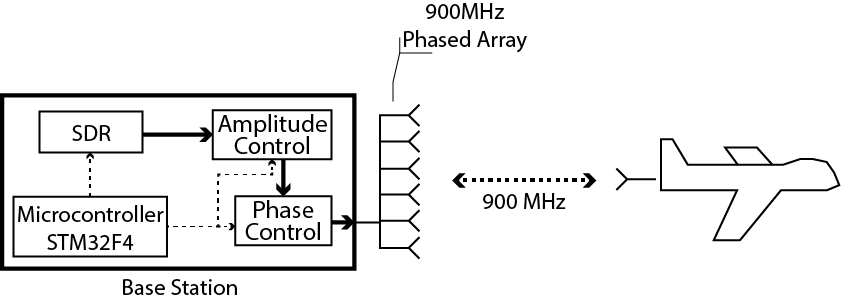
\includegraphics[]{HardwareBlockDiagram.png}
		\caption{Hardware Block Diagram \label{fig:HardwareBlockDiagram}}
	\end{figure}
	\subsection{Product Perspective}
	
		\subsubsection{System Interfaces}
			\begin{itemize}\itemsep1pt
				\item 
			\end{itemize}	
			
		\subsubsection{User Interfaces}
			\begin{itemize}\itemsep1pt
				\item 
			\end{itemize}
			
		\subsubsection{Hardware Interfaces}
			\begin{itemize}\itemsep1pt
				\item \textbf{STM32F4} -- 
				\item \textbf{Xeta SDR} -- 
				\item \textbf{Phased Array} -- 
			\end{itemize}
			
		\subsubsection{Software Interfaces}
			\begin{itemize}\itemsep1pt
				\item 
			\end{itemize}
			
		\subsubsection{Communications Interfaces}
			\begin{itemize}\itemsep1pt
				\item 
			\end{itemize}
			
		\subsubsection{Memory}
			\begin{itemize}\itemsep1pt
				\item 
			\end{itemize}
		
		\subsubsection{Operations}
			\begin{itemize}\itemsep1pt
				\item 
			\end{itemize}
		
	\subsection{Product Functions}
	
		\subsubsection{High Priorities}
		
		\subsubsection{Medium Priorities}
		
		\subsubsection{Low Priorities}
		
	\subsection{User Characteristics}
	
	\subsection{Design Constraints}
	
	\subsection{Assumptions and Dependencies}
	
\end{document}
